\documentclass[12pt]{article}
\topmargin        -0.5 in        % margins are relative to the default of 1 inch
\textheight      9.25 in
\oddsidemargin   0.0 in            % this is for pages 1, 3, 5, ...
\evensidemargin  0. in            % this is for pages 2, 3, 6, ...+++
\voffset		 0.0 in
\hoffset		 0.0 in
\textwidth       7.5 in
\headheight         0.0 in            % we don't have a running head nor
\headsep            0.0 in            % any extra space between head and text
\footskip			0.0 in
\parindent          0 pt
\usepackage[latin1]{inputenc}
\usepackage[english]{babel}
\usepackage{graphics,amssymb,amsmath,latexsym,graphicx,amsthm,mdwlist,multicol,multirow, enumerate,extsizes,setspace}
\usepackage[margin=.5in]{geometry}
%\usepackage{fancyhdr}
\usepackage[usenames]{color}
\newtheorem{theorem}{Theorem}
\newtheorem{lemma}{Lemma}
\newtheorem{definition}{Definition}
\newtheorem{ex}{Example}
\newcommand{\DS}{\displaystyle}
%\pagestyle{fancy}   

\begin{document}

\begin{center}
 \large{\underline{Chpt 7: Spanning Trees and Kruskal's Algorithm}}
\end{center}

\underline{HW}: 1, 3, 21a, 21c, 23a, 23c, 29, 31, 33, 35, 41, 49
\vspace{.1in}

\begin{definition} Network

A network is another name for a \underline{connected graph}. In the context of networks, vertices are called \underline{nodes} and edges are called \underline{links}. A network is called \underline{simple} if it does not have loops or multiple edges connecting a pair of vertices. 

\end{definition}
\vspace{.1in}

\begin{ex} TV Service

A cable TV service will be set up on one large university campus. The graph below shows the possible links that might be included in the network. The weights of each edge show the cost in hundreds of thousands of dollars to create that particular link. 

\begin{center}
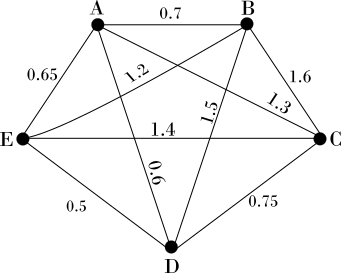
\includegraphics[width=2.5in]{ex1}
\end{center}

To send video between two locations, a direct cable link is not necessary because it is possible to send a video indirectly via another site. Therefore, sending a video from A to C could be achieved by sending the video from A to B, from B to E, and from E to C, provided the links AB, BE, and EC are part of the network.\\ 


We assume that the cost of relaying a video, compared with the cost of the direct communication link, is so small that we can neglect this amount. The problem that concerns us, therefore, is to provide service between any pair of locations in a way that minimizes the total cost of the links.\\


\begin{multicols}{2}

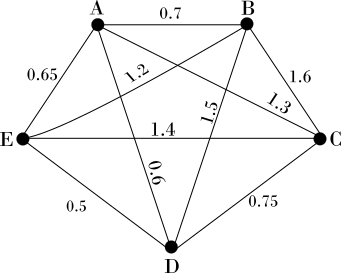
\includegraphics[width=2.5in]{ex1}

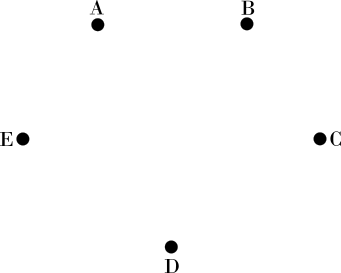
\includegraphics[width=2.5in]{ex1a}

\end{multicols}


\end{ex}




\pagebreak
%%%%%%%%%%%%%%%%%%%%%%%%%%%%%%%%%%%%%%%%%%%%%%%%%%%%%%%%%%%%
\begin{definition} Tree

A tree is a \underline{minimally connected} network. Every edge (or link) is necessary to keep the graph connected. That is, every edge is as a \underline{bridge}. A tree forms a subgraph of the original graph. Trees do not need to include every node but it must be connected. (To be minimally connected, circuits cannot be formed.)

\end{definition}
\vspace{.1in}

\begin{definition} Spanning Tree

A subgraph that is a tree and that contains (or spans) all the nodes in the original graph is called a spanning tree of the original graph.

\end{definition}


\begin{ex} Identifying Trees and Spanning Trees

Determine if the following represent a tree, a spanning tree or is not a tree.


% \begin{multicols}{2}
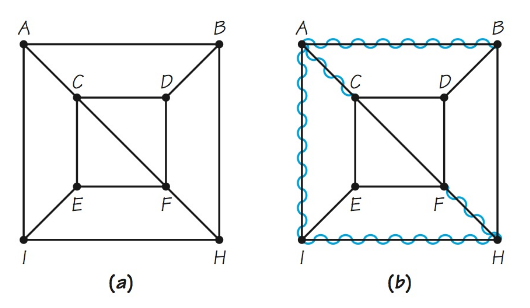
\includegraphics[width=3in]{ex3} \hspace{.1in} 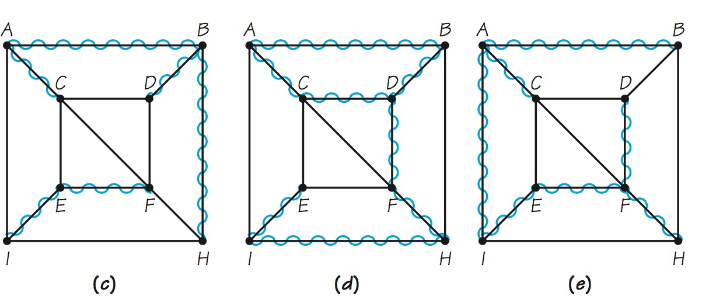
\includegraphics[width=4in]{ex3a}
% \end{multicols}

\end{ex}

\vfill


\begin{definition} Minimum Cost Spanning Tree (MST)

A spanning tree whose edge weights sum to a minimum value.
\end{definition}



\begin{definition} Kruskal's Algorithm for Minimum Cost Spanning Trees

Add links in order of cheapest cost, so that:

\begin{itemize}
\item
no circuits are formed

\item
every vertex belongs to some link added
\end{itemize}

\end{definition}

\vspace{.1in}

\begin{ex} Applying Kruskal's Algorithm

\begin{multicols}{2}

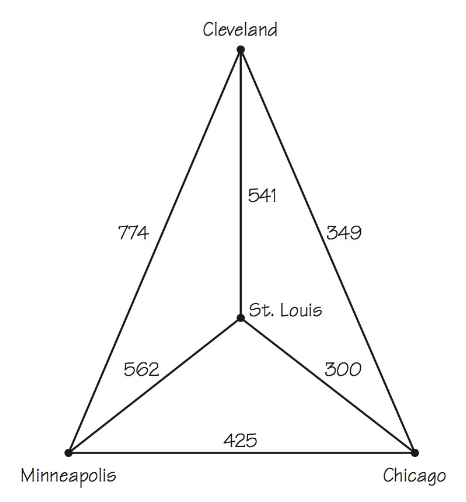
\includegraphics[width=2in]{ex4}


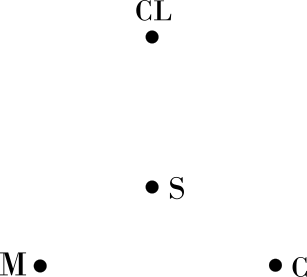
\includegraphics[width=2in]{ex2}

\end{multicols}

\end{ex}



\pagebreak
%%%%%%%%%%%%%%%%%%%%%%%%%%%%%%%%%%%%%%%%%%%%%%%%%%%%%%%%%%%%%%%%%%%%
\underline{Note:} The result of Kruskal's Algorithm:

\begin{itemize}

\item
formed a \textbf{tree}- consists of one piece and contains no circuits

\item
contains all the vertices of the original graph.

\end{itemize}

\vspace{.1in}


\begin{ex} Construction Cost

The following graph represents construction costs for roads in between houses. What is the minimum cost spanning tree for the graph? 

% 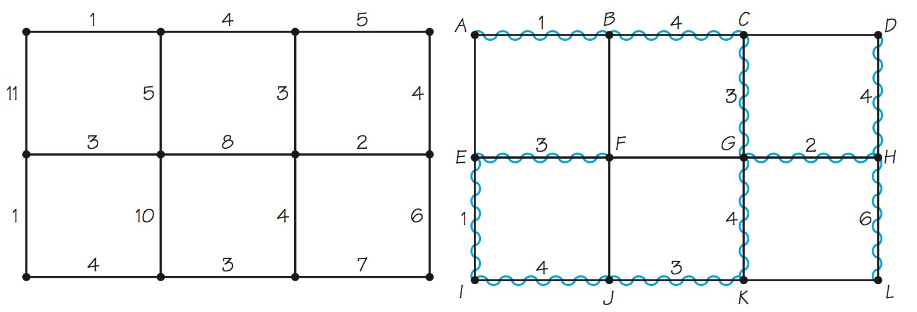
\includegraphics[width=6in]{ex5}

\begin{center}
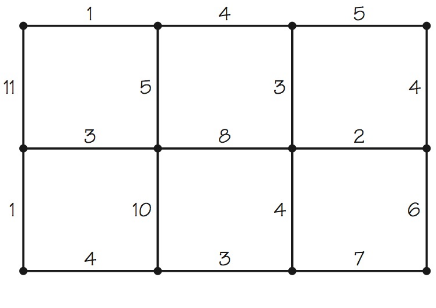
\includegraphics[width=3in]{ex5a}
\end{center}

\end{ex}


\vspace{3.75in}

\underline{Question:} We saw with the sorted edges method for constructing a Hamiltonian circuit, that the circuit created many not be the minimum cost circuit. Does Kruskal's algorithm generate the minimum cost spanning tree?

\vspace{.1in}

\underline{Answer:} YES, Kruskal showed that the \underline{greedy algorithm} described does yield the minimum answer. His work paved the way for modern infrastructure. (A greedy algorithm builds up a solution piece by piece, always choosing the next piece that offers the most obvious and immediate benefit.)

\pagebreak


\begin{ex} Minimum Cost Spanning Tree for a TSP graph.\\

A salesperson must travel to five destinations for meetings. Below is the cost of traveling to each city. Using Kruskal's algorithm, draw a minimum cost spanning tree for this situation. \\

\begin{tabular}{|c|c|c|} \hline

From	&	To		&	Cost \\ \hline
Atlanta	&	Boston	&	185   \\ \hline
Atlanta	&	Chicago	&	119   \\ \hline
Atlanta	&	Dallas	&	152   \\ \hline
Atlanta	&	Evansville	&	133   \\ \hline
Boston	&	Chicago	&	121   \\ \hline
Boston	&	Dallas	&	150   \\ \hline
Boston	&	Evansville	&	200   \\ \hline
Chicago	&	Dallas	&	174   \\ \hline
Chicago	&	Evansville	&	120   \\ \hline
Dallas	&	Evansville	&	199   \\ \hline

\end{tabular}
\end{ex}
\vfill


\begin{center}
\underline{Degrees of Separation}
\end{center}

In a connected graph, there must be at least one path connecting each vertex to every other vertex. Usually, we are interested in the shortest path connecting any two vertices. The length of the shortest path connecting two vertices is called the \underline{degree of separation} of the two vertices.

\vspace{.1in}

\underline{Activity}: Six Degrees of Separation posits that any two people in the world are connected by six or less degrees of separation.

\vspace{.1in}


\end{document}